\documentclass[a4paper,10pt]{article}
\usepackage[utf8]{inputenc}
\usepackage[T5]{fontenc} % Hỗ trợ tiếng Việt tốt nhất trên Overleaf
\usepackage[vietnamese]{babel}
\usepackage[margin=2cm]{geometry}
\usepackage{setspace}
\usepackage{enumitem}
\usepackage{sectsty}
\usepackage{xcolor}
\usepackage{hyperref}
\usepackage{graphicx}
\setstretch{1}

\sectionfont{\color{blue!60!black}\Large}
\subsectionfont{\color{blue!50!black}\large}

\title{\vspace{-1.5cm}\textbf{\huge ĐỀ XUẤT DỰ ÁN: EDUVISION}\\[0.2cm] \Large Hệ thống giám sát và phân tích tương tác lớp học thông minh bằng AI}
\author{\textbf{Đơn vị thực hiện:} Nhóm 1 \\ Nguyễn Hoàng An, Nguyễn Thành Toàn, Trần Xuân Tùng, \\ Lê Hoàng Minh Tuấn, Vương Duy Hải Nam, Phạm Anh Đức}
\date{}

\begin{document}
\maketitle
\vspace{-1cm}

\section*{1. Tóm tắt Dự án - Abstract}
EduVision là một dự án phát triển một hệ thống giám sát và phân tích tương tác lớp học tự động bằng các mô hình Deep Learning. Sử dụng dữ liệu hình ảnh trích xuất từ camera góc cao, hệ thống sẽ thực hiện điểm danh tự động, phát hiện và theo dõi trạng thái học tập của sinh viên. Kết quả phân tích sẽ được tổng hợp để tạo báo cáo đánh giá chất lượng buổi học, hỗ trợ nhà trường đưa ra các đánh giá toàn diện nhất

\section*{2. Mục tiêu Dự án - Objectives}
\begin{itemize}[noitemsep]
    \item \textbf{Tự động hóa:} Ứng dụng Face Recognition để nhận diện sinh viên vào đầu giờ học.
    \item \textbf{Bảo vệ quyền riêng tư:} Ẩn danh hóa dữ liệu hành vi trong quá trình học, chỉ giữ lại định danh ở bước điểm danh đầu giờ.
    \item \textbf{Giám sát toàn diện:} Sử dụng các kiến trúc Convolutional Neural Networks (CNN) để phát hiện đối tượng (Object Detection) và nhận diện các tư thế, hành vi.
    \item \textbf{Phân tích \& Đánh giá:} Tự động tạo báo cáo chất lượng lớp học dựa trên dữ liệu thực tế.
\end{itemize}

\section*{3. Phạm vi Triển khai - Scope}
\begin{itemize}[noitemsep]
    \item \textbf{Đối tượng sử dụng:} Sinh viên, Giảng viên, Nhà trường và Phòng quản lý.
    \item \textbf{Không gian áp dụng:} Các phòng học tiêu chuẩn, phòng thực hành (lab), và phòng thi.
\end{itemize}

\section*{4. Phương pháp \& Kiến trúc hệ thống - Methodology \& Architecture}

\begin{figure}[h]
    \centering
    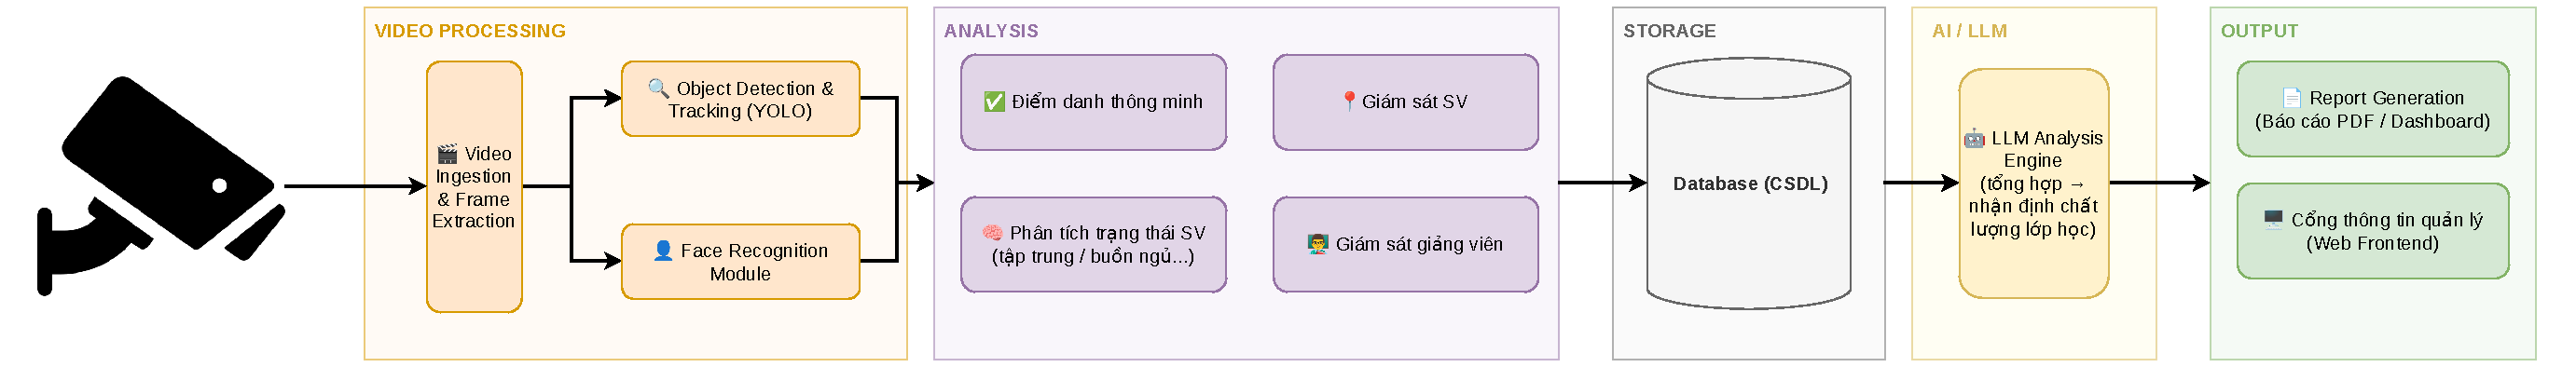
\includegraphics[width=1\textwidth]{DPL.drawio.pdf}
    \caption{Hệ thống vận hành theo chuỗi xử lý dữ liệu khép kín thời gian thực}
    \label{fig:Hệ thống vận hành theo chuỗi xử lý dữ liệu khép kín thời gian thực}
\end{figure}
\section*{5. Các Tính năng Cốt lõi - Core Features}
Hệ thống bao gồm 6 phân hệ chính:
\begin{itemize}[noitemsep]
    \item \textbf{Hệ thống Điểm danh Thông minh:} Nhận diện khuôn mặt để tự động ghi nhận thời gian vào/rời lớp và phân loại chính xác các trạng thái: có tham gia, vắng mặt, đi trễ, về sớm, hoặc không xác định.
    \item \textbf{Theo dõi Vị trí Thời gian thực:} Định vị sinh viên liên tục để phát hiện các trường hợp đổi chỗ, rời khỏi lớp học quá thời gian quy định nhằm tránh tình trạng điểm danh hộ.
    \item \textbf{Phân tích Trạng thái Sinh viên:} Ứng dụng Computer Vision để đánh giá tư thế nhằm xác định các trạng thái: tập trung, mất tập trung, buồn ngủ, làm việc riêng.
    \item \textbf{Giám sát Hoạt động Giảng viên:} Nhận diện và thống kê thời lượng giảng viên có mặt, giảng bài, tương tác với sinh viên hoặc vắng mặt.
    \item \textbf{Phân tích Chuyên sâu (AI/LLM):} Tổng hợp dữ liệu tương tác từ sinh viên và giảng viên, sử dụng mô hình LLM để chuyển đổi các thông số kỹ thuật thành các nhận định chất lượng lớp học.
    \item \textbf{Cổng Thông tin Quản lý (Frontend):} Giao diện trực quan cung cấp sơ đồ lớp học, trạng thái, danh sách điểm danh và các bảng báo cáo đánh giá.
\end{itemize}

\end{document}